\subsection{Dificultades y Contratiempos}

Durante el proceso de diseño de la placa de circuito impreso se presentaron múltiples inconvenientes inesperados que tuvieron que ser resueltos para poder concretar un diseño de circuito impreso funcional. Muchos de estos inconvenientes estuvieron dados por falta de experiencia en el ámbito de diseño de PCB y utilización de software EDA, como también por problemas de disponibilidad de algunos de los componentes seleccionados a la hora del diseño circuital de la plataforma.\\

\subsubsection{Cambio de Componentes}

\lipsum[1]\\

\subsubsection{Placa Adaptadora}

\lipsum[2]\\

\begin{figure}[h]
    \centering
    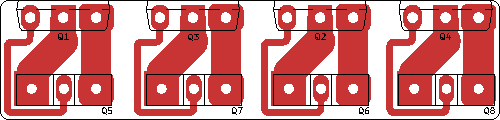
\includegraphics[scale=1.3]{Imagenes/Placa Adaptadora.pdf}
    \caption{Capa de cobre de la placa adaptadora diseñada para mitigar el error de diseño.}
    \label{fig:placa_adaptadora}
\end{figure}